\section{Способы пополнения генерируемой модели сведениями, не заданными явно во входных описаниях}
%\label{ocl-translation}

Чтобы была возможность извлечь типы из описания предметной области, она должна содержать соответствующую информацию, и в секции требований (\texttt{:requirements}) должно быть указано \texttt{:typing}. 
Если информации о типах в описании нет, то высказывать какие-либо предположения о типах объектов и аргументов действий невозможно.
В этом случе, все они будут типа \texttt{object}, базового для PDDL и все они будут транслироваться в UML-класс \texttt{Object} (рис. \ref{img:tr-untyped}).

\translation{
\begin{alltt}
(:predicates
  (hungry ?phi)
  (hasLeft ?phi)
  (left ?phi ?fork)
  ...
)
(:action getLeft
  :parameters (?p1 ?p2 ?f)
  ...
) 
\end{alltt}
}
{0.7}
{tr-untyped}
{Трансляция в случае отсутствия информации о типах}
{img:tr-untyped}


Как уже говорилось ранее, транслированные PDDL-выражения с предикатами, которые преобразуются в ассоциации с неограниченными кратностями концов, выглядят громоздко и с ними сложно оперировать. Поэтому, имеет смысл определить кратности ассоциаций более точно.
В этом может помочь только новая информация: не представленная явно в описании предметной области и задач планирования, но неявно в ней присутствующая, или пришедшая извне, например, от пользователя.

Во многих предметных областях и задачах существуют неявные ограничения на мощности концов, которые связаны прежде всего с требованиями/изменениями унарных предикатов в действиях. 
Этим изменениям сопутствуют изменения бинарных предикатов. 
Таким образом, если при анализе действий удастся выявить действия (или пары действий), которые по унарному предикату в предусловии взаимно исключают друг друга и одновременно с этим изменяют один и тот же бинарный предикат, то можно с большой уверенностью предположить, что этот бинарный предикат имеет ограниченную мощность.

\translation{
\begin{alltt}
(:action getLeft
  :parameters 
    (?p1 - Philosopher 
     ?p2 - Philosopher ?f - Fork)

  :precondition 
    (and (left ?p1 ?f)
         (right ?p2 ?f) 
         \textit{(hungry ?p1)}
         \textit{(not (hold ?p2 ?f))}
    )
      
  :effect
    (and (hasLeft ?p1)
         \textit{(hold ?p1 ?f)}
         \textit{(not (hungry ?p1))}
    )
)
\end{alltt}
}
{0.7}
{tr-assoc-1-m}
{Восстановление кратности из описания действия \texttt{[0..1]}}
{img:tr-assoc-1-m}

Более формально это можно описать следующим образом.
Предположим, что действие $a = \langle Pre_a, Effect_a \rangle$ описано в типичном для STRIPS стиле, т.е.:
\begin{center}
$Pre_a = \langle Pre_a^-, Pre_a^+ \rangle = \neg Pre_a^- \cup Pre_a^+ $,\\
$Pre_a^-, Pre_a^+ \subset Atoms_a$, \\
$Effect_a = \langle Effect_a^-, Effect_a^+ \rangle = \neg Effect_a^- \cup Effect_a^+$, \\
$Effect_a^-, Effect_a^+ \subset Atoms_a$,\\
\end{center}
где $Atoms_a$~--- множество всех фактов обо всех объектах, доступных для использования в действии $a$. $Pre_a^-, Pre_a^+$ представляют собой ограничение на состояние: одни факты должны быть истины (присутствуют в состоянии), а другие~--- точно ложны (отсутствуют в состоянии), или, что тоже самое, истинны отрицания этих атомов.
Истинность фактов, которые не упоминаются, не имеет значения. 
$Effect_a^-, Effect_a^+$~--- это факты, которые удаляются и добавляются к состоянию после применения действия, соответственно.
Если $Pre_a^+ \cap Effect_a^- \not= \emptyset$ или $Pre_a^- \cap Effect_a^+ \not= \emptyset$, что эквивалентно $I = Pred_a \cap \neg Effect_a \not = \emptyset$ и при этом $I$ содержит факт об унарном предикате, то анализируем действие дальше. 
Надо рассмотреть факты о предикатах, которые затрагивают один и тот же объект, если такие факты существуют, то можно сделать предположение о кратностях противоположных концов. Рассмотрим сказанное выше на примере действия \texttt{getLeft} из предметной области ``Обедающие философы''(рис.~\ref{img:tr-assoc-1-m}).

У данного действия в предусловии проверяется предикат \texttt{hungry}, а в эффекте этот же предикат удаляется.
Посмотрим, какие изменения сопутствуют изменению этого предиката.
Одновременно с ним меняется предикат \texttt{hold} с неизменным вторым вторым аргументом \texttt{?f}. 
Можно предположить, что противоположный конец \texttt{philosopher} соответствующей ассоциации имеет кратность не более 1.

Кроме такого анализа действий можно предложить анализировать задачи для предметной области. 
Если набор задач будет достаточно хорошим, то на основании того, какие в задачах даются начальные условия, можно выдвинуть предположения о мощностях ассоциаций. 
\begin{wrapfigure}{r}{0.4\linewidth}
{\centering
    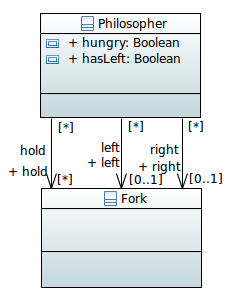
\includegraphics[width=\maxwidth{0.9\linewidth},keepaspectratio]{tr-assoc-m-1}
    \caption{Восстановление кратности из задачи планирования}\label{img:tr-assoc-m-1}
}
\end{wrapfigure}
В задаче, представленной на рис.~\ref{img:its-states}, для все той же предметной области видно, что каждый философ имеет не более одной вилки справа и не более одной вилки слева от него (на самом деле, в точности одну), поэтому можно предположить соответствующую кратность у ассоциаций \texttt{left} и \texttt{right}, как показано на рисунке \ref{img:tr-assoc-m-1}.

Разрабатываемый инструмент может предлагать пользователю в интерактивном режиме утверждать или отвергать данные предположения.
Если предположение утверждено~--- то учесть его при трансляции ассоциаций и выражений. 
Если предположение отвергнуто~--- то можно выдвинуть другое предположение (например, более слабое), а если предположений не осталось~--- оставить неограниченную мощность у ассоциации.

%%%%%%%%%%%%%%%%%%%%%%%%%%%%%%%%%%%%%%%%%%%%%%%%%%%%%%%%%%

%Если не удалось получить информацию о кратностях концов, то предполагается наиболее общий случай \texttt{[*]}. \tabularnewline



% Как правило, в предусловиях действий и в описаниях начальных состояний задач указывается большое количество утверждений об атомах (положительных или отрицательных), поэтому получившееся после трансляции OCL-выражение будет выглядеть довольно громоздким и плохо обозримым. Но с этим ничего нельзя поделать, если никак не удастся ограничить кратности концов ассоциации.

Предположим, что для бинарного предиката удалось каким-либо образом ограничить кратность второго конца ассоциации \texttt{argName2} хотя бы до \texttt{[0..1]}. Тогда основные логические выражения будут транслироваться несколько проще. Это отображено в таблице ниже:
\\

{
    \renewcommand{\arraystretch}{1.3}
    \small
    \centering
    \ttfamily
    \begin{tabular}{|p{0.35\linewidth}|p{0.60\linewidth}|}
        \hline
        \normalfont\bfseries PDDL\:-выражение & \normalfont\bfseries OCL\:-выражение \\
        \hline
          (pred arg1 arg2) & arg1.argName2 = arg2 \\
        \hline
          (not (pred arg1 arg2)) & arg1.argName2 <> arg2\\
        \hline
          (pred arg1 ... argN) 
          & 
          arg1.argName2 = arg2 and ...\newline
          \rule{2em}{0em} and arg1.argNameN = argN \\
        \hline
          (not (pred arg1 ... argN))
          &
          arg1.argName2 <> arg2 or ...\newline
          \rule{2em}{0em} or arg1.argNameN <> argN \\
        \hline

    \end{tabular}
}
\\[5pt]



%Итак, напомним, что PDDL-эффект описывает изменения объектов в результате применения действия в некотором состоянии. UML-постусловие действия задает логическое ограничение на состояние после применения действия. Для этого может использоваться конструкция OCL \texttt{@pre}.


